\documentclass[onecolumn, draftclsnofoot,10pt, compsoc]{IEEEtran}
\usepackage{url}
\usepackage{setspace}
\usepackage{graphicx}
\usepackage{epstopdf}
\epstopdfsetup{update} % only regenerate pdf files when eps file is newer
\usepackage[utf8]{inputenc}
\usepackage[english]{babel}
\usepackage{indentfirst}
\usepackage{geometry}
\usepackage{color}
\usepackage{tikz}
\usepackage{rotating}
\usepackage{pgfgantt}
\usepackage{xcolor}
\geometry{textheight=9.5in, textwidth=7in}


\newganttchartelement{orangebar}{
    orangebar/.style={
        inner sep=0pt,
        draw=red!66!black,
        very thick,
        top color=white,
        bottom color=orange!80
    },
    orangebar label font=\slshape,
    orangebar left shift=.1,
    orangebar right shift=-.1
}

\newganttchartelement{bluebar}{
    bluebar/.style={
        inner sep=0pt,
        draw=purple!44!black,
        very thick,
        top color=white,
        bottom color=blue!80
    },
    bluebar label font=\slshape,
    bluebar left shift=.1,
    bluebar right shift=-.1
}


% 1. Fill in these details
\def \CapstoneTeamName{		MAV Challenge}
\def \CapstoneTeamNumber{		32}
\def \GroupMemberOne{			Justin Sherburne}
\def \GroupMemberTwo{			Kaiyuan Fan}
\def \GroupMemberThree{			Yingshi Huang}
\def \CapstoneProjectName{		AHS Micro-Air Vehicle Challenge}
%\def \CapstoneSponsorCompany{	Columbia Helicopters}
\def \CapstoneSponsorPerson{		Nancy Squires, Ph.D.}

% 2. Uncomment the appropriate line below so that the document type works
\def \DocType{		%Problem Statement
				%Requirements Document
				%Technology Review
				Design Document
				%Progress Report
				}
			
\newcommand{\NameSigPair}[1]{\par
\makebox[2.75in][r]{#1} \hfil 	\makebox[3.25in]{\makebox[2.25in]{\hrulefill} \hfill		\makebox[.75in]{\hrulefill}}
\par\vspace{-12pt} \textit{\tiny\noindent
\makebox[2.75in]{} \hfil		\makebox[3.25in]{\makebox[2.25in][r]{Signature} \hfill	\makebox[.75in][r]{Date}}}}
% 3. If the document is not to be signed, uncomment the RENEWcommand below
%\renewcommand{\NameSigPair}[1]{#1}

%%%%%%%%%%%%%%%%%%%%%%%%%%%%%%%%%%%%%%%
\begin{document}
\begin{titlepage}
    \pagenumbering{gobble}
    \begin{singlespace}
    	
\includegraphics[height=4cm]{coe_v_spot1}
        \hfill 
        % 4. If you have a logo, use this includegraphics command to put it on the coversheet.
        %\includegraphics[height=4cm]{CompanyLogo}   
        \par\vspace{.2in}
        \centering
        \scshape{
            \huge CS Capstone \DocType \par
            {\large\today}\par
            \vspace{8pt}
            \textbf{\Huge\CapstoneProjectName}\par
			\vspace{1.5in}
            {\large Prepared for}\par
            % \Huge \CapstoneSponsorCompany\par
            % \vspace{5pt}
            {\Large\NameSigPair{\CapstoneSponsorPerson}\par}
			\vspace{3pt}
            {\large Prepared by }\par
            Group\CapstoneTeamNumber\par
            % 5. comment out the line below this one if you do not wish to name your team
            \CapstoneTeamName\par 
            \vspace{8pt}
            {\Large
                \NameSigPair{\GroupMemberOne}\par
                \NameSigPair{\GroupMemberTwo}\par
                \NameSigPair{\GroupMemberThree}\par
            }
            \vspace{.5in}
        }
        \begin{abstract}
        The purpose of this document is to elaborate on design concepts related to the implementation of the Micro Air Vehicle project. Our goal is to provide our intended audience with information on the design and implementation of our core features. Here we will outline technical concerns and viewpoints contained within the scope of the Micro Air Vehicle project. 
        \end{abstract}     
    \end{singlespace}
\end{titlepage}
\newpage
\pagenumbering{arabic}
\tableofcontents
% 7. uncomment this (if applicable). Consider adding a page break.
\listoffigures
%\listoftables
\clearpage


\section*{Revision History}

\begin{center}
    \begin{tabular}{|c|c|c|c|}
        \hline
		Name & Date & Reason For Changes & Version\\
        \hline
		Design Document & Nov 29, 2017 & Initial Creation & 1.0\\
		\hline 
    \end{tabular}
\end{center}




\section{Overview}


\subsection{Scope}% of the document

This document is intended to inform the reader of the technical goals of the Micro Air Vehicle Challenge project. Here we will describe subcomponents of the project, and how each subcomponent will be implemented into the overall design. It will provide a clear framework for each piece, and provide viewpoints on how each element will be designed. It is not a definition of requirements, or a concrete time line of events leading up to the completion of the project.


\subsection{Purpose}% of the document

The purpose of this document is to describe how our project will be implemented to accomplish the tasks defined by the AHS 6th annual MAV challenge. The goal of this project is to create a remotely piloted helicopter with an autonomous flight feature. This document will explain the details of the project's design.


\subsection{Intended Audience}

The intended audience of this design document is project team members, project sponsors or facilitators, and project collaborators.  

\section{Definitions} % Alphabetized?
\begin{description}
		\item{AHS} -  American Helicopter Society.
        \item{Autonomous} -  Acting independently from any controlling source.
        \item{CSI} - Camera Serial Interface. This is the primary interface for the Raspberry Pi cameras. 
        \item{ESC} - Electronic Speed Controller. Used to control motor speed with low voltage logic. 
        \item{GUI} -  Graphical User Interface.
        \item{GPIO} - General-purpose input/output.
        \item{MAV} -  Micro Air Vehicle.
        \item{USB} - Universal Serial Bus
        
\end{description}     


\section{System requirements} 


\subsection{Functional Requirements}  

\begin{itemize}
\item The vehicle must weigh less than 500 grams including the battery.
\item The vehicle must be shorter than 17.7 inches in any one dimension. 
\item The vehicle is required to operate from an electric power source.
\item It must be able to take off and land vertically, and have the ability to maintain a stable altitude (hover).
\item It must have some sort of on-board camera system featuring at least one camera.
\item It must use standard communication methods, with a preference on 2.4GHz communications.
\item It must have an emergency cutoff switch that will power off the vehicles motors in case of a loss of communication.
\item It must have a manual control override so an operator can steer the vehicle back to the competition area. 
\end{itemize}


\subsection{Non-functional Requirements} 

\begin{itemize}
\item{The vehicle should be able to navigate the competition area without human intervention.}
\item{The cameras should maintain a minimum quality of 540p at 30fps.}
\item{The image processing system should recognize each of the following objects: landing areas, packages, boundary lines, and large obstacles.}
\item{Hardware should be light enough and small enough to fit within the vehicle limitations.}
\item{WiFi communication should maintain a steady connection at a distance of more than 50 ft. }
\end{itemize}



\section{Conceptual Designs}%  for the project


\subsection{Design Overview} %Concept sketch + brief description

\begin{figure}[ht]
\centering
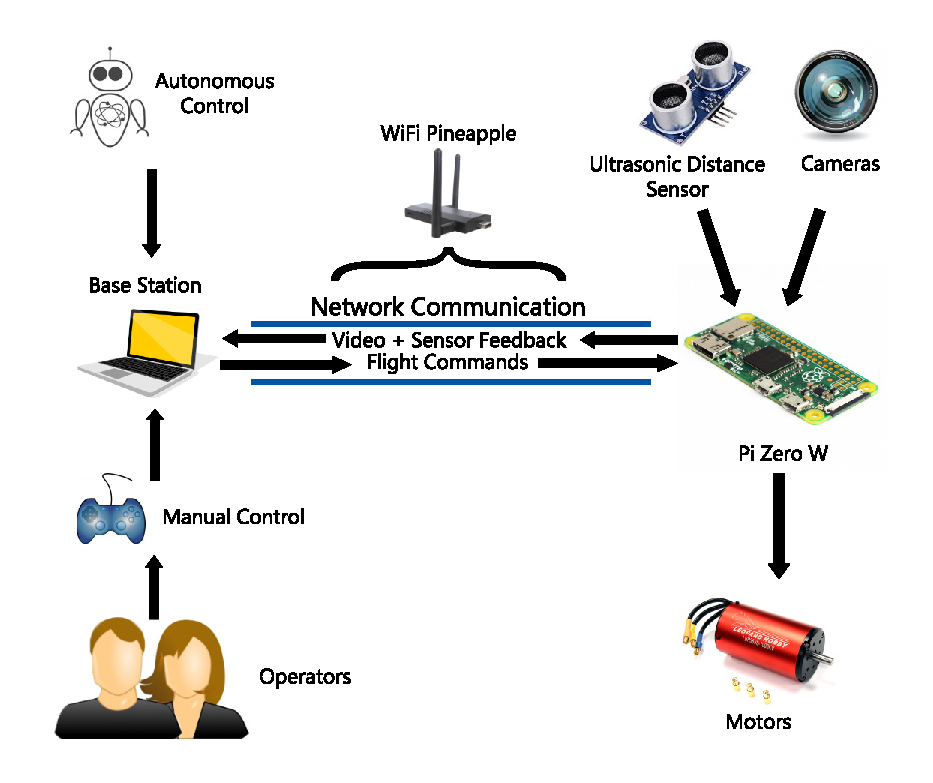
\includegraphics[height=3.5in]{DesignOverview}
\caption{Conceptual Design Overview}
\end{figure}


\subsection{Design Components}

\subsubsection{Device Communication} 

The communication between the aircraft and the base station will be connected by WiFi. Data is transferred over a 2.4GHz channel, allowing Raspberry Pi board and base station to receive and transmit data when they are in the range of a WiFi network. We will establish a WiFi network by using a router, specifically the WiFi Pineapple \cite{r12}. In the event of communication loss, the vehicle should attempt to reconnect for no more than 3 seconds. If the connection is not re-established, the vehicle will shut down the motors. 


\subsubsection{Hardware}

The two main logic control components are the base station and the Raspberry Pi \cite{r3}. These two components will be able to communicate to each other through the WiFi Pineapple router. The Base station will handle the difficult computations regarding image processing and flight planning. Additionally, the base station will be able to select between manual control mode or autonomous control mode using a GUI. The Raspberry Pi will handle motor control logic, and elevation control. Video and sensor information will be bassed from the Raspberry Pi to the base station, and directional commands will be returned from the base station to the Pi. 


\subsubsection{Flight Control}

We will connect motor controllers to the Raspberry Pi with GPIO pins. We will write a GPIO access program to access GPIO pins and establish communication with motors. We can configure the GPIO pins to start and shutdown the motors. Furthermore, we can set the logical voltages either low or high to change the speed. This code to control the motors will be able to handle commands from both manual and autonomous inputs.


\subsubsection{Sensors}% (camera + ultrasonic)

Camera Sensors are used to easily capture images. For the manual flight, the camera sensor will stream video (image frames) back to the base station. For the autonomous operation, these “images” can be used by video-processing algorithms for recognizing the target, searching the home-base, and operating the hover-hold. We will equip two cameras to our aircraft. One front Camera to process stream video and one at the bottom to find targets and the landing places.


The ultrasonic sensor can emit a specific frequency of sound waves and listen to that sound wave bounce back. The sensor can record the elapsed time between the sound wave being emitted and the sound wave bouncing back. \cite{r11} Once we know the speed of the sound wave, it is able to calculate the distance between the ultrasonic sensor and the object. we will use an ultrasonic sensor at the bottom of aircraft to detect the height from the ground and measure the boundary range.


\subsubsection{Image Processing}

All image processing will be done on the base station to increase calculation performance. Image processing should be able to distinguish four main objects: Delivery targets, packages, boundary lines, and obstacles. Once these objects are correctly identified, the autonomous system will then have to identify where that object is located in correlation to the vehicle. After a general location is established (Left, Right, in front, below, ect.) The autonomous system should then send the appropriate flight commands to the vehicle. 

\subsubsection{User Interface}

The user interface should be simple, with only the necessary information needed to control the micro air vehicle displayed. There should be a white button to enable manual flight control, as well as a red button to stop all flight commands. At minimum the front facing camera stream will be displayed on the user interface. The second camera stream may be added if computational power is not significantly compromised. Additionally, image processing overlays may also be added under the same circumstances. 



\section{Design Viewpoints} % (viewpoints are just an in-depth explanation of a certain aspect of the design)

\subsection{Introduction}  
	Viewpoints are an in-depth evaluation for each of our above design components. Here we will break each viewpoint into three primary categories: design concerns, design elements, and design examples. Design concerns address what we are trying to solve, and what problems we are anticipating to come across. Design elements will break down the specific goals of each viewpoint. Within the deign elements we will elaborate on each specific task and a general idea of how it will be implemented. In design examples we will review any existing technologies that might solve the viewpoint we are addressing. If there are no existing technologies, then we will review similar applications and explain what we are doing differently. 



\begin{center}
    \begin{tabular}{|c|p{0.3\linewidth}|p{0.4\linewidth}|}
        \hline
		Design viewpoint & Design concerns & Example Design Concepts \\
        \hline
		Communication & Reliability, Fail-safe Operations  & Video streaming applications and standard data packet transfer over WiFi.  \\
		\hline 
        Hardware & Reliable, Lightweight, Multi-functional & Raspberry pi, CSI cameras, Ultrasonic sensors, WiFi Pineapple\\
		\hline 
        Image Processing & Object Detection, Directional Translation & OpenCV \cite{r8}, Matlab Image toolbox \cite{r9}, directional markers  \\
		\hline 
        Flight Control & Motor control, Logic outline, Input Arguments  & ESC motor controller and GPIO pins.  \\
		\hline 
        Positioning & Ultrasonic Distance sensors, Image distance calculations  & OpenCV distance and positioning calculations, distance based on ultrasonic readings.  \\
		\hline 
        User control & User Interface, Manual Control Methods, Emergency Shutdown  &  Web interface attached to the base station system with basic user controls. \\
		\hline 
    \end{tabular}
\end{center}

    

\subsection{Communication Viewpoint} 
\begin{itemize}
 \item{ \textbf{Design Concerns:}}

The main design concern for communication is maintaining a low-latency, high-bandwidth connection between a base station and the vehicle. Design considerations should be made based on what will best address the above design constraint. Additional concerns about communication distance and strength will be secondary considerations for this project. \\ 

\item{ \textbf{Design Elements:}}

There are three objects that rely on steady communication channels: The base station, the vehicle, and the router. The router will act as an intermediary to the base station in order to boost the signal range, and produce a local network that the vehicle can connect to. The base station will connect to the router via USB or ethernet cable, and the vehicle will connect over the 2.4GHz wireless channel. This creates a closed network that we can easily secure to communicate from our base station to our vehicle and back. Video and Ultrasonic Sensor information will be passed from the vehicle to the base station, and the flight calculations will be returned to the vehicle for execution. \\

\item{ \textbf{Design Examples:}}

Typically MAV's are controlled using radio communication, so our approach to this is not conventional. The main reason behind this is because WiFi has limited range compared to radio communication methods. For our application we will be in relatively close proximity to the vehicle, so this makes WiFi a better option for data throughput. \\


\end{itemize}



\subsection{Hardware Viewpoint} 
\begin{itemize}
\item{ \textbf{Design Concerns:}}

Our primary concerns with heardware is being lightweight enough to fit within the constraints of our vehicle requirements, and being able to commmunicate to the vehicle reliably. We will elaborate on our hardware decisions below based on those primary requirements. Secondary considerations will be based on ease of use, and project implementation. 

\item{ \textbf{Design Elements:}}
Our hardware requirements are limited to a couple different factors. The following components are needed for our implementation: A camera, a distance sensor, a base station, a router, and a vehicle controller. The vehicle controller is our most constrained object because it is limited by our sive and weight limitations. This is why we decided to use the Raspberry pi zero. This computer is one of the most powerful computer for it's size on the market, and it is extremely inexpensive. Our camera was also decided base on this choice because is was specifically designed for the CSI input for the raspberry pi. The router (WiFi Pineapple) is based on what was on hand, but it also has the added benifit of not needing an external power source. The base station can be implemented on any laptop as long as it is capable of running Ubuntu or another Lunix distribution.  

\item{ \textbf{Design Examples:}} %If there are any!

Our design is typical of any server-client relationship. Our base station will act as the sever, while the vehicle is acting as the client. The client (vehicle) relays information from their data sources back to the server. The server will then perform the difficult computations that the client is not capable of handling. There is an intermidiary, the router, which is also found in any client-server relationship. This element is less documented, but equally as critical to the overall success of the project.
\end{itemize}


\subsection{Image Processing Viewpoint}
\begin{itemize}
\item{ \textbf{Design Concerns:}}

The concerns of image processing can be separated into two parts: object detection and directional translation. During competition, the object to be detected is the envelop with two colors which are white and red. The envelop might not be in the original video range at the beginning of our flight, so the detection depends on the path of vehicle. During flight, the angle of the cameras will be changing. This causes the view of object to also change. Positions and shapes can increase the difficulty of detecting the object. The directional translation component is based on the relative location within the images recived by the cameras. The view from cameras alone cannot estimate exact distances, so sensor and mathematic calculation based on known sizes can decrease the deviation. \\

\item{ \textbf{Design Elements:}}

At the start of the flight, the cameras will capture video. The video data will send to the base station via WiFi router. If the software cannot discover the object, then it will continue to move around the environment. If the object in the range of camera, base station will calculate a path to pick up the package. According to the path, the vehicle will convert this path into movements. On the way to pick up the object, the microhelicopter will avoid any obstacle it encounters. The base station will keep track of movements and make sure the microhelicopter arrives at the package pick up place. The microhelicopter will then pick up the envelop and attempt to bring it to the corresponding distination. \\ 
\item{ \textbf{Design Examples:}} %If there are any!

In roder to process images, the vehicle needs a program that can handle streaming video in an efficent manner. OpenCV and Matlab Image toolbox can accomplish this task. However, OpenCV is an open source library, while Mathlab is a licensed product (which is available to students for free). OpenCV is focuses more on the object detection so it is a better choice.\\
\end{itemize}



\subsection{Flight Control Viewpoint} %(how do we talk to the motors)
\begin{itemize}
\item{ \textbf{Design Concerns:}}

The main design concern for flight control is maintaining a stable connection between the Raspberry Pi with the multiple ESC motor controllers and motors. Additional concerns will be ESC motor controllers sending the correct pulsing signals to motors with the commands received from the users. \\
\item{ \textbf{Design Elements:}}

Flight control will be accomplished through connecting the ESC motor controllers with the Raspberry Pi through the GPIO pins. Then, we will have each ESC motors controllers with each motor and with an extended power bank. We will write a GPIO access program to enable the GPIO pins to write outputs to the ESC motor controllers, then proceed to signal the motors. Once the connection completed, users can control the flight by sending the command to the Raspberry Pi board.\\

\item{ \textbf{Design Examples:}} %If there are any!

There are many examples of this using typical radio communicaions to controll air vehicles. These are low-latency algorithms used to convert simple directional inputs into frequency based control algorithms for the ESC controllers. \\

\end{itemize}



\subsection{Positioning Viewpoint} %(distance + camera positioning)
\begin{itemize}
\item{ \textbf{Design Concerns:}}

The concern for positioning are the measurement accuracy of the ultrasonic sensor and the deviation between the realistic distance with the distance calculated by the image processing algorithm.\\
\item{ \textbf{Design Elements:}}

Camera sensors and ultrasonic sensors will be implemented to measure distance. If we know the dimension of an object and we can use it as a reference to the image that collected by the camera sensor. Distance can be calculated with various of algorithms using OpenCV. The ultrasonic sensor should be connected to the Raspberry Pi through the GPIO pins. Ultrasonic sensors can measure the distance to the ground by emitting specific frequency of sound waves and recording the elapsed time untill sound wave bouncing back.\\
\item{ \textbf{Design Examples:}} %If there are any!

Distance from camera to object can be calculated through trianglulation similarity. \cite{r13} If we have an object with a known width W. We have initial distance from the object to the camera. Given the initial image collected by the camera sensor, we can measure the pixel width of the object in the image via OpenCV, marked as P. The focal F can be calculated as F = (P * D) / W. Then new distance D’ can be measured with the new pixel width in the later image. The formula will be D’ = (W * F) / P.\\
\end{itemize}



\subsection{User Control Viewpoint}% (how do we talk to the pi, talk about GUI)
\begin{itemize}
\item{ \textbf{Design Concerns:}}

The User interface should display 4 things. 2 video feeds, a amunal override, and a emergency stop. The second window camera interface is completely optional becuse it is only needed for flight object recognition. The function bottons will take priorety ofer the second window for a camera stream. \\
\item{ \textbf{Design Elements:}}

This is an interface required for the user to control the moicrohelicopter through the base station controller. The user will have control through an external controller for forward, backwards, up, down, left , and right. The user control interface also needs to be able to attached with web interface. \\ 
\item{ \textbf{Design Examples:}} %If there are any!

The phsical controller can be a illustion for the user interface. Every controller should include all the basic functions needed, like turn left or right and move forward and backward. Our different derections should be represented by individual keys on the controller. And the emergency shutdown should be accessable through the controller or the user interface on the base station.
\end{itemize}


\section{Conclusion}

The Micro Air Vehicle challenge not only encompasses the design requirements listed above, but also the design requirements put forth by the Electrical and Mechanical sub-teams. While this design document provides a comprehensive coverage of the logical systems required, there are additional contributions that are not specified above. This document adequately outlines the design requirements for the Computer Science sub-team attached to Oregon State University's Micro Air Vehicle Challenge team. 


\bibliographystyle{IEEEtran}
\bibliography{references}

\newpage

\section{Timeline}

\begin{rotate}{270}
\begin{ganttchart}[
    hgrid style/.style={black, dotted},
    vgrid={*5{black,dotted}, *1{white, dotted}, *1{black, dashed}},
    x unit=.8mm,
    y unit chart=9mm,
    y unit title=12mm,
    time slot format=isodate,
    group label font=\bfseries \Large,
    link/.style={->, thick}
    ]{2017-10-04}{2018-06-21}
    \gantttitlecalendar{year, month=name}\\

    \ganttgroup[
        group/.append style={fill=blue}
    ]{System Build}{2017-10-04}{2018-5-12}\\ [grid]
	
    \ganttbluebar[
        name=Communications
    ]{Communications}{2017-10-07}{2017-11-12}\\ [grid] 
	
    \ganttbluebar[
    	name=Motor Control
    ]{Motor Control}{2017-11-12}{2018-01-15}\\ [grid]   
	
    \ganttbluebar[
    	name=Flight Control
    ]{Flight Control}{2018-1-11}{2018-02-30}\\ [grid]    
	
    \ganttbluebar[
    	name=User Interface
    ]{User Interface}{2017-12-12}{2018-3-13}\\ [grid]
	
    \ganttbluebar[
    	name=Image Recognition
    ]{Image Recognition}{2017-12-12}{2018-3-13}\\ [grid]

    \ganttbluebar[
    	name=Integration Testing
    ]{Integration Testing}{2018-3-13}{2018-5-12}\\ [grid]

    \ganttgroup[
        group/.append style={fill=orange}
    ]{Competition}{2017-11-9}{2018-05-16}\\ [grid]
	
    \ganttorangebar[
        name=Design proposal
    ]{Design proposal}{2017-11-20}{2018-01-30}\\ [grid]
	
	\ganttorangebar[
        name=Final Selection
    ]{Final Selection}{2018-01-30}{2018-03-17}\\ [grid]
	
	\ganttorangebar[
        name=Event Participation
    ]{Event Participation}{2018-05-12}{2018-05-16}\\ [grid]
    
    \ganttgroup[
        group/.append style={fill=green}
    ]{Expo}{2018-05-16}{2018-06-15}\\ [grid]
    
\end{ganttchart}
\end{rotate}







\end{document}
